\newpage 

\section{Cost of Electricity} 

 Contributors to LCOE projections are given by: 
 \begin{equation} 
 LCOE [\$ MWh] = \frac{(C_{AC} + (C_{OM} + C_{F})(1+y)^Y)}{(8760.P_E.p_a)} 
 \label{eq:coe}
\end{equation} 
where C$_{AC}$ [USD/year] is the annual capital cost charge (entailing the total capital cost of the plant (TCC (USD) multiplied by the Fixed Charge Rate (FCR (/year)), C$_{OM}$ [USD/year] is the annual operations and maintenance cost, C$_{SCR}$ [USD/year] is the annual scheduled component replacement costs, C$_{F}$ [USD/year] is the annual fuel costs, $y$ is the annual fractional increase in fuel costs over the expected lifetime of the plant $Y$ [years], P$_{E}$ [MWe] is the net electric power of the plant, p$_{a}$ is the plant availability (typically 0.6-0.9).  A small charge used to be imposed to build up a fund to cover end-of-life Decontamination and Decommissioning ($DD$), f$_{DD}$ (USD/kWh), but the DD costs are now included in the direct capitalized costs (Cost Category 58), so are omitted here.

\subsection{Cost Category 70: Annualized O\&M Cost (AOC)}

The Operations and Maintenance (O\&M) costs was previously estimated to be 2 \% of the direct cost, assessed annually.  The O\&M cost depends on the system complexity and the requirements of regulations, security and maintenance. The costs are computed based on look-up tables, such as the one shown in Fig. \ref{fig:statista} at 60 USD per kilowatt-year.  

\begin{figure}[b!] 
\centering 
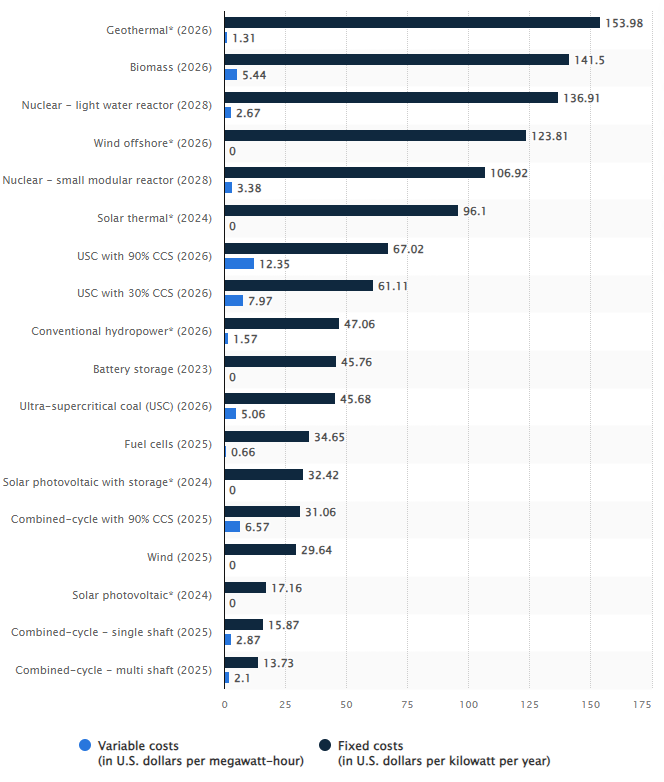
\includegraphics[scale=0.5]{StandardFigures/statista.png} 
\caption{Operations and Maintenance costs for various kinds of power plants.} 
\label{fig:statista} 
\end{figure} 

\begin{verbatim} 
C_OM = 60 * PE * 1000 = C700000  
\end{verbatim} 

Annualized O\&M costs are \$ C700000 M.

\subsubsection*{Cost Category 71 – O\&M Staff}
Component in the financial structuring of operational expenditures in various industries, especially those involving significant infrastructure and machinery, such as power generation, manufacturing, and utilities.  The costs under Cost Category 71 predominantly include:

\begin{itemize}
    \item \textbf{Salaries:} The regular wages paid to the O\&M staff.
    \item \textbf{Training and Development:} Costs associated with professional development, training programs, and certifications to ensure staff is up-to-date with the latest operational and maintenance practices.
    \item \textbf{Overtime and Shift Allowances:} Compensation for extended work hours and shift differentials, especially in 24/7 operational setups.
\end{itemize}

Cost Category 71 is crucial in operational budgeting due to:

\begin{enumerate}
    \item \textbf{Staffing Optimization:} The need for an optimal number of skilled staff to ensure efficient and safe operations.
    \item \textbf{Direct Impact on Operational Efficiency:} The performance and availability of O\&M staff directly affect operational uptime and efficiency.
    \item \textbf{Regulatory Compliance:} Compliance with labor laws and industry-specific regulations regarding staffing and worker safety.
\end{enumerate}

\textit{Cost Category 71 – O\&M Staff} encompasses all aspects of costs related to the personnel responsible for the operation and maintenance of facilities. Efficient management of this category is vital for ensuring operational excellence, staff well-being, and overall financial health of the organization.


\subsubsection*{Cost Category 72 – Management Staff}
Crucial aspect of operational expenses in various sectors, especially in industries where effective management plays a pivotal role in ensuring efficient operations and achieving organizational objectives.  Cost Category 72 typically encompasses:

\begin{itemize}
    \item \textbf{Salaries:} The basic remuneration paid to operations management staff.
    \item \textbf{Bonuses and Incentives:} Performance-related bonuses and incentives that align management objectives with corporate goals.
    \item \textbf{Professional Development:} Expenses related to the continuous learning and development of management skills, including workshops, seminars, and courses.
    \item \textbf{Leadership Training:} Specific training focused on enhancing leadership qualities necessary for effective management.
\end{itemize}

The inclusion of Cost Category 72 in operational expenditure is significant due to:

\begin{enumerate}
    \item \textbf{Strategic Decision Making:} Management staff play a crucial role in strategic decision-making and operational planning.
    \item \textbf{Operational Efficiency:} Effective management is key to ensuring operational efficiency and organizational success.
    \item \textbf{Staff Leadership:} Management staff are responsible for leading, guiding, and motivating the workforce, directly impacting productivity and morale.
\end{enumerate}

\textit{Cost Category 72 – Management Staff} is integral to the financial planning of any organization, particularly in operational contexts. It involves not just the direct costs of salaries and benefits but also the broader implications of effective management on organizational performance and success.

\subsubsection*{Cost Category 73 – Salary-Related Costs}
This Cost Category includes taxes, insurance, fringes, benefits, and any other annual salary-related costs.

\subsubsection*{Cost Category 74 – Operations Chemicals, and Lubricants}

\subsubsection*{Cost Category 75 – Spare Parts}
Critical element in the operational budgeting of various industries, particularly in sectors that rely on continuous and efficient machinery and equipment operation.  This cost category encompasses:

\begin{itemize}
    \item \textbf{Operational Spare Parts:} Expenses associated with spare parts used in regular operations. These do not include major equipment or capital plant upgrades.
    \item \textbf{Exclusion of Capitalized Items:} It specifically excludes items that would be capitalized or amortized over a period or quantity of product.
\end{itemize}

Cost Category 75 plays a significant role in Operations and Maintenance (O\&M) budgeting, as it:

\begin{itemize}
    \item \textbf{Ensures Operational Continuity:} Regular replacement and availability of spare parts are crucial for uninterrupted operations.
    \item \textbf{Impacts Maintenance Scheduling:} Influences the planning and scheduling of maintenance activities.
    \item \textbf{Affects Operational Efficiency:} Directly impacts the overall efficiency and lifespan of the operational equipment.
\end{itemize}

\textit{Cost Category 75 – Spare Parts} is essential for the smooth operation and maintenance of machinery and equipment in various industries. It encompasses the costs of spare parts necessary for regular operation and scheduled component replacements, playing a vital role in operational budgeting and efficiency.  Cost of any operational spare parts, excluding capital plant upgrades or major equipment that will be capitalized or amortized over some period or quantity of product.

\subsubsection*{Cost Category 76 – Utilities, Supplies, and Consumables}
Cost of water, gas, electricity, tools, machinery, maintenance equipment, office supplies and similar items purchased annually.

\subsubsection*{Cost Category 77 – Capital Plant Upgrades}
Upgrades to maintain or improve plant capacity, meet future regulatory requirements or plant life extensions.

\subsubsection*{Cost Category 78 – Taxes and Insurance}
Property taxes and insurance costs, excluding salary related.

\subsubsection*{Cost Category 79 – Contingency on Annualized O\&M Costs}
This Cost Category includes an assessment of additional cost necessary to achieve the desired confidence level for the annualized O\&M costs not to be exceeded.

\subsection{Cost Category 80: Annualized Fuel Cost (AFC)}

%\subsection{Annual Fuel Cost} 
The fuel cost, C$_{F}$, is calculated as follows.  The unit cost of deuterium as D2 is 3,700 \$/kg; deuterium contributes negligibly to the COE of a fusion power plant. In the long run, the power plant is self-sufficient in terms of tritium fuel production because of the breeding capability of the blanket so that no specific tritium-fuel charge is reported. It should be recognized, however, that there is a significant cost for tritium in the direct cost of the D-T fueled fusion reactor, represented in Cost Category 22.05 Fuel Handling and Storage. Cost of the primaryC and secondaryC coolant is included in Cost Category 27 Special Materials.\\

Consists of:  
\begin{verbatim} 
m_D = 3.342*10^(-27) # (kg)
u_D = 2175 #Where u_D ($/kg) = 2175 ($/kg) 
C_F = N_mod * P_NRL * 1e6 * 3600 * 8760 * u_D * m_D * p_a / (17.58 * 1.6021e-13)
\end{verbatim} 

Total annual fuel costs are \$ C800000 M per year.

\subsubsection*{Cost Category 81 – Refueling Operations}
This Cost Category includes incremental costs associated with refueling operations.

\subsubsection*{Cost Category 84 – Fuel}
This Cost Category includes annualized costs associated with the fuel cycle.

\subsubsection*{Cost Category 86 – Processing Charges}
This Cost Category includes storage and processing if fuel is brought in from offsite.

\subsubsection*{Cost Category 87 – Special Nuclear Materials}
This Cost Category covers materials such as heavy water, sodium, lead, helium, or other energy transfer mediums that are required on an annual basis. It includes costs associated with disposal or treatment if necessary. 

\subsubsection*{Cost Category 89 – Contingency on Annualized Fuel Costs}
This Cost Category includes an assessment of additional cost necessary to achieve the desired confidence level for the annualized fuel costs not to be exceeded.

\subsection{Cost Category 90: Annualized Financial Costs (AFC)}


Consists of: Capital recovery factor (or constant dollar FCR), $f_{cr}$ multiplied by the total capital cost. This is a function of the cost of money and the period over which the investment must be paid off (see 2019 NETL report \cite{NETL2019a}). In this case, it is the lifetime of the plant, plifetime years, plus the construction time, constructionTime years. Thus, the capital recovery factor is calculated from 

\begin{equation}
    C(x,N) = \frac{x(1+x)^N}{(1+x)^N-1} = \left[ \sum_{n=1}^N \frac{1}{(1+x)^N}] \right] ^{-1},
    \label{eq:C}
\end{equation}

where 

\begin{equation}
    x = i_cf_c + i_pf_p +(1-t)i_df_d
\end{equation}

is the effective cost of money. Here, $i_c$ is the rae of return on common stock, $f_c$ is the fraction of capital form common stock, $i_p$ is the rate of return of preferred stock, $f_p$ is the fraction of capital from preferred stock, $i_d$ is the nterest rate on deb, and $f_d$ is the capital from debt. 

From here, the fixed charge rate can be calculated as 
\begin{equation}
    f_{cr} = \frac{Ck}{(1-t)} - \frac{td}{(1-t)} + t_p + r,
\end{equation}

where $C$ is the capital recovery factor (\ref{eq:C}), $k$ is the adjustment for investment tax credit, $t$ is the effective income tax rate, $d$ is the levelized tax depreciation, $t_p$ is the property tax rate and $r$ is the levelized interim replacement cost. For this power plant, see \ref{tab:ec_vals} for values. Applying these calculations to this power plant with a lifetime of plifetime yields $f_{cr} = $ fcr.\\


\begin{table}
    \centering
    \begin{tabular}{cc|cc}
    \hline
      $N$ (plant life)  & plifetime & $t$ (construction period) & constructionTime\\
       $i_c$  & 0.1 & $t_p$ (property tax rate)& 0\\
        $i_p$ & 0 & $x_1$ (pre-tax)& 0.073\\
        $i_d$ & 0.05 & $x$ (post-tax)& 0.065\\
        $f_c$ & 0.45 & $x_r$ (real)& 0.045\\
        $f_p$ & 0 & $k$ & 1\\
        $f_d$ & 0.55 & $C(x,N)$ & 0.077\\
        $i$ (general inflation) & 0.02 & $C(x_r,N)$ & 0.061\\
        $e$  (escalation)& 0.02 & $r$ (interim replacement)& 0\\
        $e_r$ (real escalation) & 0 & $f$ (depreciable fraction of TCC)& 0.881\\
        $t_s$ (income tax 1) & 0.06 & $d$ (levelized depreciation)& 0.036\\
        $t_f$ (income tax 2) & 0.21 & $f_{cr}$ & 0.0910\\
        $t$ (effective income tax) & 0.257 & $f_{cr0}$ & 0.0722\\
    \hline    
    \end{tabular}
    \caption{Values used in calculation of capital recovery factor  $f_{cr}$, the effective cost of money, $x$, and the fixed charge rate, $R$.}
    \label{tab:ec_vals}
    \label{tab:my_label}
\end{table}

By multiplying the capital recovery factor, $f_{cr}$ by the total capital cost, $C_{99}$, the annual capital cost charge is calculated.
Annualized Financial Costs are \$ C900000 M.

\subsubsection*{Cost Category 91 – Escalation}
Critical financial concept often used in the planning and analysis of long-term projects, particularly in industries such as energy or construction. This category accounts for the changes in costs over time due to factors like inflation, market dynamics, and changes in labor or material costs. Escalation is the systematic increase in costs over the life of a project. It is distinct from \textit{contingency}, which is used to cover unforeseen costs. Escalation accounts for known, predictable changes in cost such as:

\begin{itemize}
    \item \textbf{Inflation:} General increase in prices and fall in the purchasing value of money.
    \item \textbf{Market Fluctuations:} Changes in costs due to supply and demand dynamics.
    \item \textbf{Labor Cost Changes:} Variations in labor costs due to economic conditions or labor market changes.
    \item \textbf{Material Cost Variations:} Fluctuations in the cost of raw materials.
\end{itemize}

In many financial estimates, particularly initial cost assessments, Cost Category 91 is often excluded. This exclusion is typically because:

\begin{enumerate}
    \item \textbf{Simplification:} To simplify the early stages of financial planning.
    \item \textbf{Variability:} Due to the unpredictable nature of some escalation factors.
\end{enumerate}

While often excluded from initial estimates, escalation is crucial in:

\begin{itemize}
    \item \textbf{Business Plans:} For a realistic long-term financial outlook.
    \item \textbf{Financing Proposals:} To present a complete picture to potential investors or lenders.
    \item \textbf{Regulatory-Related Documents:} Where detailed, realistic cost projections are required.
\end{itemize}

Effective management of Cost Category 91 involves:

\begin{enumerate}
    \item \textbf{Regular Reassessment:} Continuously updating the project's cost estimates to reflect current economic conditions.
    \item \textbf{Risk Mitigation:} Developing strategies to mitigate the impact of negative cost escalations.
    \item \textbf{Informed Decision Making:} Using escalation estimates to make informed financial and strategic decisions.
\end{enumerate}



\subsubsection*{Cost Category 92 – Fees}
This Cost Category primarily encompasses the costs associated with annual fees necessary for the operation of such facilities.  Fees under Cost Category 92 typically include, but are not limited to, costs related to:

\begin{itemize}
    \item \textbf{Licensed Reactor Processes:} These are fees paid for obtaining and maintaining the licenses required for reactor operation. They cover regulatory compliance and safety standards as set by nuclear regulatory bodies.
    \item \textbf{Nuclear Operating License Fees:} Fees associated with the acquisition and renewal of operating licenses for nuclear facilities. These are critical for legal and safe operation.
    \item \textbf{Regulatory Compliance:} Fees related to ensuring compliance with various environmental, safety, and operational regulations.
    \item \textbf{Inspection and Oversight:} Costs incurred for regular inspections and oversight activities by regulatory authorities to ensure adherence to safety and operational guidelines.
\end{itemize}

\textit{Cost Category 92 – Fees} is an essential financial Cost Category, especially for nuclear facilities, where regulatory compliance and licensing play a critical role. Proper management and allocation of funds for these fees are vital for uninterrupted and legal operation.

\subsubsection*{Cost Category 93 – Cost of Money}
The \textbf{cost of money} is akin to the \textit{opportunity cost} of using capital for a specific purpose. When capital is allocated to operating costs, it is an alternative to investing that capital elsewhere. Thus, the cost of money represents the return that this capital could have earned if invested differently.
\begin{itemize}
    \item Sources of Capital. Capital for operating costs can be sourced either externally or from within the organization (retained earnings). External financing includes loans, bonds, or other forms of borrowing, incurring interest payments. Retained earnings are internal funds saved and not distributed as dividends, carrying an opportunity cost as these funds could be used elsewhere.
    \item Impact on Operating Costs. In financial Cost Categorying, the cost of money is considered an \textit{indirect cost} of operating. It reflects the financial charges incurred due to the company's capital structure, including both the direct costs (e.g., interest on loans) and the opportunity costs (e.g., using retained earnings).
    \item Project Financing and Cost of Capital.  For large-scale projects like nuclear power plants, the cost of money is crucial in project financing. The strategy (debt vs. equity) and the corresponding costs of capital significantly affect the overall project economics.
    \item Risk and Return Considerations. The cost of money reflects the project's risk profile. Higher-risk projects lead to higher costs of capital, as lenders and investors demand higher returns for increased risks.
    \item Long-term Implications.  For long-term projects, the cost of money impacts the project's \textit{net present value} (NPV) and \textit{internal rate of return} (IRR). Effective management of the cost of money is essential for the project's long-term financial viability.
    \item Dynamic Nature.  The cost of money changes with market conditions, economic environment, and the organization's financial health. This necessitates continuous monitoring and reevaluation of financing strategies.
\end{itemize}

\textbf{In summary}, Cost Category 93 - Cost of Money - encompasses the financial implications of the capital used for operating costs. It includes both direct costs (like interest payments) and indirect costs (like opportunity costs of capital). Proper management of this Cost Category is crucial for the economic feasibility and financial health of large-scale projects.




\subsubsection*{Cost Category 99 – Contingency on Annualized Financial Costs}
This Cost Category includes an assessment of additional costs necessary to achieve the desired confidence level for the annualized financial costs not to be exceeded, including schedule uncertainties. Not included here.


\subsection{Levelized Cost of Electricity} 

\begin{table}[h!] 
\begin{tabular}{l c c } 
Net electric power & MW & PNET \\
Plant availability & \% & PAVAIL \\
Inflation & \% & yinflation \\
Lifetime of plant & Years & lifeY \\
Capital cost, $C_{AC}$ &     M\$/annum    &    C900000      \\ 
Operations and Maintenance Costs, $C_{OM}$ & M\$/annum  &      C700000 \\ 
Fuel Costs, $C_{F}$ & M\$/annum  &       C800000 \\ 
    \end{tabular} 
    \caption{Cost components in the LCOE calculation.}
    \label{tab:lcoe} 
\end{table} 

Following equation \ref{eq:coe}, the LCOE is C1000000 \$/MWh or C2000000 c/kWh. 

%\subsection{Levelized Cost of Electricity Nth of a Kind (NOAK)}  

%It is possible to distinguish between the First of a Kind (FOAK) power plant, which might function as a Demo, and more mature 10th of a Kind (TOAK), the latter incorporating learning credits in the COE estimate, consistent with U.S. fusion-reactor design-community practice. The ARIES study, like STARFIRE \cite{BAK80} and most other U.S. fusion-reactor designs reported in the last decade, assumes FPC unit costs consistent with these learning-curve \cite{Hir64,Arg90} credits, rather than first-of-a-kind unit costs (including R\&D) appropriate for ITER \cite{Ite89} or some other reported designs \cite{Coo89b}. An 80 \% learning curve ({\it {\it i.e.},} 0.80 progress ratio, $p$), as used for ARIES, represents the expectation that each doubling of production represents a \hbox{$p\simeq$ 0.8} reduction in unit costs. A tenth-of-a-kind reactor represents, nominally, $\simeq$3.3 doubling of production or $p^{(ln 10/ln 2)}\simeq$ 50 \% cost reduction relative to first-of-a-kind FPC costs.  Of course, the actual production experience varies \cite{Arg90}.  Learning credits are not applied to BOP items, consistent with mature industrial production in which the learning credits have already been wrung out.  For similar reasons, a 94 \% learning curve is recommended for advanced fission cost estimates \cite{Del93}.   